\usetikzlibrary{arrows}
\definecolor{ccffff}{rgb}{0.8,1.,1.}
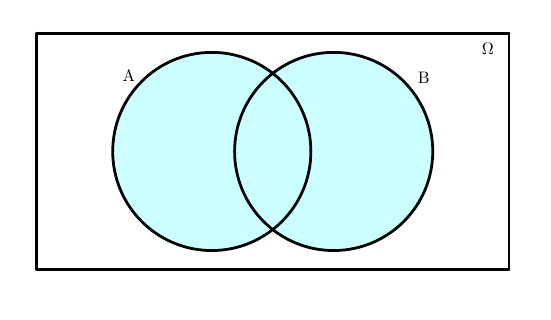
\begin{tikzpicture}[line cap=round,line join=round,>=triangle 45,x=1.0cm,y=1.0cm, scale=0.6,every node/.style={scale=0.6}]
\clip(-0.1870638729100964,-0.46671950332886286) rectangle (10.301322760748397,5.120090328019539);
\draw [line width=1.pt,color=ccffff,fill=ccffff,fill opacity=1.0] (3.7100909661527863,2.5) circle (2.1cm);
\draw [line width=1.pt,color=ccffff,fill=ccffff,fill opacity=1.0] (6.289909033847214,2.5) circle (2.1cm);
\draw [line width=1.pt] (0.,0.)-- (0.,5.);
\draw [line width=1.pt] (0.,5.)-- (10.,5.);
\draw [line width=1.pt] (10.,5.)-- (10.,0.);
\draw [line width=1.pt] (10.,0.)-- (0.,0.);
\draw (9.3,4.910199129935732) node[anchor=north west] {$\Omega$};
\draw (1.7,4.35460478206683) node[anchor=north west] {A};
\draw (7.949306688103378,4.29904534727994) node[anchor=north west] {B};
\draw [line width=1.pt] (6.289909033847214,2.5) circle (2.097024222769593cm);
\draw [line width=1.pt] (3.7100909661527863,2.5) circle (2.097024222769593cm);
\end{tikzpicture}
